\documentclass[a4paper,titlepage,openright,12pt]{report}
\usepackage{amsmath}
\usepackage{amssymb}
\usepackage{amsthm}
\usepackage[toc]{appendix}
\usepackage{array}              
\usepackage{captcont}
\usepackage{enumerate}
\usepackage{fancyhdr}                              
\usepackage{float}
\usepackage{graphicx}    
\usepackage{hyperref}
\usepackage{lipsum}
\usepackage{makeidx}
\usepackage{moreverb}
\usepackage{multirow}
\usepackage{rotating}
\usepackage{setspace} 
\usepackage[font=footnotesize]{subfig}
\usepackage{supertabular}
\usepackage{tabularx}
\usepackage{tikz}
\usepackage{titlesec}
\usepackage[nottoc,notlot,notlof]{tocbibind}     
\usepackage{url}
\usepackage{verbatim}
%\usepackage{epsfig}   
%\usepackage[toc,page]{appendix}
%\usepackage[algoruled]{algorithm2e}
%\usepackage[figure,algoruled]{algorithm2e}
%\usepackage[figure,boxruled]{algorithm2e}

%\newtheorem{theorem}{Theorem}
%\newtheorem{corollary}[theorem]{Corollary}
%\newtheorem{conjecture}[theorem]{Conjecture}
%\newtheorem{lemma}[theorem]{Lemma}
%\newtheorem{proposition}[theorem]{Proposition}
%\newtheorem{definition}[theorem]{Definition}
%\newtheorem{Example}[theorem]{Example}
%\newtheorem{axiom}{Axiom}
%\newtheorem{remark}{Remark}
%\newtheorem{exercise}{Exercise}[section]
%\newtheorem{fact}[theorem]{Fact}
%\newtheorem{property}[theorem]{Property}
\setlength{\parindent}{0pt}%for paragraph spacing
\setlength{\parskip}{1ex plus 0.5ex minus 0.2ex}
\setlength{\textheight}{8.5in}
\pagestyle{fancy}
% with this we ensure that the chapter and section
% headings are in lowercase.
%\renewcommand{\bibname}{References}

\DeclareRobustCommand{\rchi}{{\mathpalette\irchi\relax}}
\newcommand{\irchi}[2]{\raisebox{\depth}{$#1\chi$}} % inner command, used by \rchi

\renewcommand{\chaptermark}[1]{\markboth{#1}{}}
\renewcommand{\sectionmark}[1]{\markright{\thesection\ #1}}
\fancyhf{} % delete current setting for header and footer
\fancyhead[LE,RO]{\bfseries\thepage}
\fancyhead[LO]{\bfseries\rightmark}
\fancyhead[RE]{\bfseries\leftmark}
%\rfoot{\bfseries\thepage}
\cfoot{\em $\copyright$ 2014, Indian Institute of Technology Delhi}
\renewcommand{\headrulewidth}{0.5pt}
\renewcommand{\footrulewidth}{0.5pt}
\addtolength{\headheight}{2.5pt} % make space for the rule

\fancypagestyle{plain}{%
\fancyhead{} % get rid of headers on plain pages
\fancyfoot{}
%\rfoot{\bfseries\thepage}
\cfoot{\em $\copyright$ 2014, Indian Institute of Technology Delhi}
\renewcommand{\headrulewidth}{0pt} % and the line
}

%% The smart version of cleardouble page.
\let\origdoublepage\cleardoublepage
\newcommand{\clearemptydoublepage}{%
  \clearpage
  {\pagestyle{empty}\origdoublepage}%
}

\let\cleardoublepage\clearemptydoublepage


\date{}


\addtolength{\oddsidemargin}{30pt}
\addtolength{\evensidemargin}{-40pt}

\titlespacing*{\chapter}{0pt}{-50pt}{20pt}
\titleformat{\chapter}[display]{\normalfont\huge\bfseries}{\chaptertitlename\ \thechapter}{20pt}{\Huge}
% \DeclareGraphicsExtensions{.pdf,.png,.jpg,.ps}
\floatstyle{boxed} 
\restylefloat{figure}
\setcounter{lofdepth}{2}
\setcounter{lotdepth}{2}

\newtheorem{claim}{Claim}[section]
\newtheorem{theorem}{Theorem}[section]
\newtheorem{defn}{Definition}[section]
\newtheorem{fact}{Fact}[section]

\graphicspath{{./Figures/}}
\makeindex
\makeatletter
\setlength{\@fptop}{0pt}
\makeatother
\begin{document}

%\begin{comment}
% Begin title page
\pagenumbering{roman}
\begin{titlepage}
\begin{center}

%\LARGE{\textsf{\bfseries ENTER YOUR THESIS TITLE HERE}}\\
\LARGE{\bfseries Improving Video Activity Recognition using Markov Logic Networks}\\
\vspace{20pt}
\normalsize
\emph{A thesis submitted in partial fulfillment} \\
\emph{of the requirements for the degree of} \\
\vspace{20pt}
\bfseries MASTER OF TECHNOLOGY \\
\vspace{20pt}
\emph {in}\\
\vspace{20pt}
\bfseries Computer Science \& Engineering \\
\vspace{20pt}
\emph {by}\\
\vspace{20pt}
\Large{\bfseries Niranjan Viladkar} \\
{\normalsize {\bfseries Entry No. 2012MCS2810}}\\
\ \\
%\ \\
{\normalsize \emph {Under the guidance of}}
\ \\
\Large{\bfseries Dr. Parag Singla} \\
\ \\
\vspace{30pt}
%\begin{center}

\includegraphics[scale=0.2]{iit_logo.pdf} \\
\vspace{10pt}
%\end{center}
\large{\textsc{Department of Computer Science and Engineering,\\
Indian Institute of Technology Delhi.\\ May 2014.}}
\end{center}
\end{titlepage}

%\newpage
%\cleardoublepage
\onehalfspacing
\thispagestyle{empty}

\normalfont
\begin{center}
\LARGE{ Certificate} 
\end{center}

\vspace{0.5in}

This is to certify that the thesis titled {\bfseries Improving Video Activity Recognition using Markov Logic Networks} being submitted by
{\bfseries Niranjan Viladkar} for the award of {\bfseries Master of Technology} in {\bfseries Computer Science \& Engineering} 
is a record of bona fide work carried out by him under my guidance and supervision at the {\bfseries Department of Computer Science \& Engineering}. 
The work presented in this thesis has not been submitted elsewhere either in part or full, for the award of any other degree or diploma.

\vspace{1.5in}

\underline{\hspace{5cm}}\\
{\bfseries Dr. Parag Singla} \\
{\bfseries Department of Computer Science and Engineering} \\
{\bfseries Indian Institute of Technology, Delhi}\\ 

\thispagestyle{empty}
\begin{center}
\LARGE{Acknowledgments} 
\end{center}

\vspace{0.5in}

%Replace \lipsum with your acknowledgement
\lipsum[1]

\vspace{1.5in}

{\bfseries YOUR NAME}

\thispagestyle{empty}


% \setcounter{page}{1}
\thispagestyle{empty}
\begin{center}
\LARGE{Abstract}
\end{center}

\vspace{0.5in}

%replace \lipsum with your abstract
Human Activity Recognition is an important vision problem. 
Most existing appraoches ( TODO -cite) perform classification of video clips 
based on low level features like HoG-HoF. They don't consider the domain knowledge while classification.
This methodology is vulnerable to noisy training data.

For example, presence of two persons in a clip increases chances of activity `conversation',
but low level features may not be able to capture this effectively.

This project adds domain knowledge in the form of object and people information
to the classification using Markov Logic. Markov Logic caputres semantic relationship
using weighted first order logic formulae. Thus the model learnt is less vulenrable to noisy
training data.

This project gives an end to end system for activity recognition. It takes input from 
a video classifier and an object detector and builds semantic model on top of this information.
Activity predictions using this approach shows improvement over the existing frameworks.


\thispagestyle{empty}
%\begin{center}
\LARGE{Acknowledgments} 
\end{center}

\vspace{0.5in}

%Replace \lipsum with your acknowledgement
\lipsum[1]

\vspace{1.5in}

{\bfseries YOUR NAME}


\thispagestyle{empty}
\setcounter{tocdepth}{1}
\tableofcontents

\thispagestyle{empty}

\listoffigures

\listoftables
%\end{comment}

\thispagestyle{empty}
\cleardoublepage
\onehalfspacing
%%%%%%%%%%%%%%%%%%%%%%%%%%%%%%%%%%%%%%%%%%%%%%%%%%%%%%%%%%%%
 
%\setcounter{page}{1}
\pagenumbering{arabic}

%You may have as many chapters as you please. This is just for reference.

\chapter{Introduction}

\label{ch1_INTRO}

%Replace \lipsum with text.
% You may have as many sections as you please. This is just for reference.





Human activity recognition is an area of interest in the field of vision.
For example, if one wants to extract only a certain type of activity
sequence from YouTube videos, like eating or driving etc., a highly accurate and precise 
video recognition system would drastically reduce the need for human intervention.
The work in \cite{improving} processes YouTube dataset for activity recognition problem.

\begin{comment}
This project tries to improve the existing activity recognition system
by adding semantic information about the domain and support for uncertainty to it.
\end{comment}

Existing activity recognition systems \cite{actionsInContext,Realistic,improving}  do not take advantage of underlying domain.
Domain may have significant influence over the activity types, the objects appearing
in the activity etc. For example, presence of a dining table improves the chances
of activity eating as compared to driving. Or if, the video is occluded partially,
but objects like bottle and chair are visible, then also, chances of activity eating
are more as compared to other activities. This relationship between objects and activities
can be captured by First Order Logic (FOL).

But merely using FOL is not sufficient. In its basic form, FOL uses hard constraints.
To explain this with example, consider a rule
\begin{equation}
	\label{MLNRule}
	\forall clip ~ HasObject( clip, bottle ) \implies HasActivity( clip, eating )
\end{equation}

In real world scenario, it is perfectly possible that a video clip contains a bottle,
but the activity might be different than eating. 
The rule gets violated in this scenario as it is universally quantified over all the clips. 
Rule may also get violated in case of noisy training data. 
Thus, using hard constraints is neither practical nor robust for real world video clips. 

Solution to this is to attach weights with rules like \eqref{MLNRule} with weights being proportional to the real world relevance.
This idea can be captured using Markov Logic Networks (MLNs). Markov Logic allows us 
to capture the relationship between activities and objects using weighted first order logic formulae.
This helps in building a better overall model for activity detection.


This project exploits the semantic relationship between activities and objects
augmenting the information captured by low level features. 
Aim of this project is to provide end to end recognition system to improve 
the existing human activity recognition systems
by adding domain knowledge i.e. object and people information to them.



Chapter \ref{ch2_BACKGROUND} gives the theoretical background. It explains video classification using only video features. It explains how to extract and use the video features. 
It further describes object detection in detail and also describes the theory of Markov Logic Networks. 
Chapter \ref{ch3_RELATED} throws light on previous approaches and points out potential improvement areas.
Chapter \ref{ch4_APPROACH} explains design decisions and approach of this project.
Chapter \ref{ch5_RESULTS} shows the result comparisons.
Finally thesis concludes with chapter \ref{ch6_CONCLUSION} which notes conclusion and future work.


%\chapter{Classification using video features}

\label{ch2_STIP}

%Replace \lipsum with text.
% You may have as many sections as you please. This is just for reference.

Video clips representing human actions can be classified based on features extracted from the video.
Below sections explain what these features are and how to use them.

\section{Spatial Temporal Interest Points\index{Spatial Temporal Interest Points}}
As explained in \cite{laptev2005} spatial temporal interest points (\index{STIP}STIPs) are 3 dimensional points in 
space and time where the local video features show significant variations. 
In \cite{actionsInContext} the features extracted at STIPs are shown to perform satisfactorily for human activity recognition. 
At each STIP, \index{Histograms of Oriented Gradient}histograms of oriented gradient (HoG\index{HoG}) and \index{Histograms of Optical Flow} histograms of optical flow (\index{HoF}HoF) are evaluated.
The number of HoG and HoF features at each STIP are 72 and 90 respectively.
Concatenating vectors of HoG and HoF features, we get a single 162 element descriptor for each STIP. 

\section{Clustering}
After extraction of STIP features, each video clip roughly has $O(1000)$ such descriptors.
100,000 descriptors are sampled randomly from all the descriptors across all the clips.
While doing random sampling, each clip is given equal chance - this avoids biased sampling
towards ( or against) any particular class of videos if they happen to be longer ( or shorter) than other videos on an average.
These 100,000 random descriptors are clustered into $k = 200$ clusters using k-means.

\section{\index{Bag of Features Representation}Bag of Features Representation}
Each descriptor in each clip is clustered into one of the $k$ clusters using
least Euclidean distance. Thus each clip is represented by a $k$ sized vector
where $i^{th}$ element in this vector represents number of descriptors of that clip 
nearest to the $i^{th}$ cluster. This vector is called a Bag of Features (\index{BoF}BoF)
representation of the clip.


\begin{table}[t]
\centering
\begin{tabular}{| l | c |}
\hline
{\bf Activity Class} & {\bf Average Precision} \\ \hline
%
AnswerPhone & 11.36\% \\ \hline
DriveCar & 66.96\% \\ \hline
Eat & 45.45\% \\ \hline
FightPerson & 57.63\% \\ \hline
GetOutCar & 17.86\% \\ \hline
HandShake & 25.93\% \\ \hline
HugPerson & 15.15\% \\ \hline
Kiss & 18.18\% \\ \hline
Run & 38.78\% \\ \hline
SitDown & 40.96\% \\ \hline
SitUp & 5.26\% \\ \hline
StandUp & 35.20\% \\ \hline
Average AP & 31.56\% \\ \hline
%
\end{tabular}
\caption{Average precision for classification using only video features}
\label{table:AP_OnlyAction}
\end{table}


\section{\index{Support Vector Machines}Support Vector Machines}
The BoF representation of all training clips are used to train a
support vector machine (\index{SVM}SVM) and BoF representation of a disjoint set of testing clips is classified using
learnt model. For training a SVM model, a radial basis function (RBF) kernel is used with parameters $C = 100$ 
and $\gamma = 0.01$. A one-versus-rest learning strategy is used to learn as many models as there are action classes.
In case of this data set, there are 12 action classes and thus 12 models are learnt.

Classification using only video features are compared taking \index{Average Average Precision|see {AAP}} average average precision as a measure.
As explained in \cite{actionsInContext}, average precision(AP) approximates area under recall-precision curve.
Thus, AP for each activity class is calculated and then finally averaged over all the classes, average AP (\index{AAP}AAP) is calculated.

The table \ref{table:AP_OnlyAction} shows the APs for each individual class for classification using only video features.



%\chapter{Object Detection}

\label{ch3_OBJ}

%Replace \lipsum with text.
% You may have as many sections as you please. This is just for reference.

Video clips of certain activity class have peculiar set of objects present in it.
If one could find objects present in the video clip, the activity prediction can 
potentially be made more confident. Below sections introduce the object detection
method and its use in this project.

\section{Object Detector}
Object detector based on Discriminatively Trained Deformable Part Models \cite{voc-release4} was used in
the project. It can run on an image at a time. The detectors used in this project are trained on PASCAL 2007 data sets.
There are 20 models corresponding to 20 different objects.
These objects are : aeroplane, bicycle,
bird, boat, bottle, bus, car, cat, chair, cow, dining table, dog, horse,
motorbike, person, potted plant, sheep, sofa, train, tv monitor.
For this project only 10 relevant models were used : bicycle, bottle, bus, car,
chair, diningtable, motorbike, person, sofa, tvmonitor.

\section{Detection in Video}
Above described object detector models work on a single image at a time. To detect objects in video clips, 1 frame per second was extracted from the video clip and all the object detector models were run on the frame. In the data set used in this project, shortest clips is about 3-4 seconds long and longest clips are of the order of a minute. Frame rate is 24 frames per second.

The object detector models give a \index{Bounding Box}bounding box and a confidence (also called \index{Decision Value}decision value) for each detection 
on an absolute scale between $-\infty$ to $\infty$. 
Usually, a positive decision value represents true positive in all the models. 
A negative decision value represent lesser confident detection. 
It might be a true positive or a false positive. 
One can specify a threshold decision value before running object detector model 
so that only the detections at least as confident as the threshold are considered.
Usually, such thresholds are negative to allow detection of lesser confident objects also.

\section{Output of Object Detector}

The visual output of object detector looks as shown in figures \ref{fig:CarDetection} and \ref{fig:PersonDetection}. 
The red boxes are called as bounding boxes.
For each box, a confidence value is also evaluated - also called as decision value.

Table \ref{table:ObjDetection} shows the decision values for sample detections.

\floatstyle{plain}
\restylefloat{figure}
\begin{figure}[here]
\begin{center} 
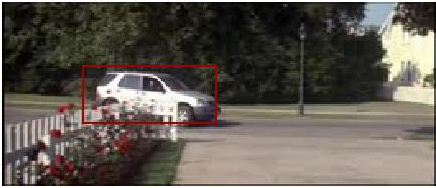
\includegraphics[scale=0.5]{car_detection_1.jpg} 
\caption{ Car detection in a frame. \label{fig:CarDetection}} 
\end{center} 
\end{figure}  

\begin{figure}[here]
\begin{center} 
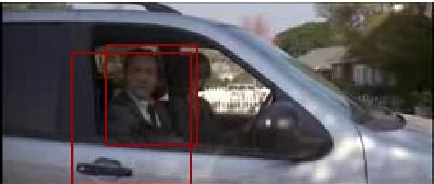
\includegraphics[scale=0.5]{person_detection_151.jpg} 
\caption{ Person detection in a frame. \label{fig:PersonDetection}} 
\end{center} 
\end{figure}  


\begin{table}[t]
\centering
\begin{tabular}{| l | c |}
\hline
{\bf Activity Class} & {\bf Average Precision} \\ \hline
%
AnswerPhone & 11.36\% \\ \hline
DriveCar & 66.96\% \\ \hline
Eat & 45.45\% \\ \hline
FightPerson & 57.63\% \\ \hline
GetOutCar & 17.86\% \\ \hline
HandShake & 25.93\% \\ \hline
HugPerson & 15.15\% \\ \hline
Kiss & 18.18\% \\ \hline
Run & 38.78\% \\ \hline
SitDown & 40.96\% \\ \hline
SitUp & 5.26\% \\ \hline
StandUp & 35.20\% \\ \hline
Average AP & 31.56\% \\ \hline
%
\end{tabular}
\caption{Average precision for classification using only video features}
\label{table:ObjDetection}
\end{table}



TODO - table showing sample output


%\chapter{Markov Logic Networks}

\label{ch4_MLN}

%Replace \lipsum with text.
% You may have as many sections as you please. This is just for reference.

As explained in \cite{MarkovLogic}, Markov Logic consists of set of First order
logic (FOL) formulae associated with weights. The FOL formulae form the structure 
of Markov Logic Networks (MLNs). Background and theory of MLNs and calculation of
weights of formula is explained in the coming sections.

\section{Markov Networks}
\index{Markov Networks}Markov Network is an undirected graph $G$ with its nodes as set of variables $X = (X_1, X_2,\ldots, X_n) \in \rchi $.
Apart from graph, it also consists of \index{Potential Functions}potential functions $\phi_k$ for each clique $k$ in the graph.
Potential function $\phi_k$ is a real valued function of the state of $k^{th}$ clique.
The joint distribution is given by

\begin{equation}
	\label{jointDist}
	P(X = x) = \frac{1}{Z}{\displaystyle \prod_{k} \phi_{k}(x_{\{k\}})}
\end{equation}

where $x_{\{k\}}$ is the state of $k^{th}$ clique;
$Z$, also known as \index{Partition Function}partition function, is given by

\begin{equation}
	\label{partitionFunc}
	Z = \displaystyle \sum_{x \in \rchi} \displaystyle \prod_{k} \phi_k(x_{\{k\}}) 
\end{equation}

If clique potentials are replaced by exponentiation of weighted sum of features of state,
joint distribution can be given as

\begin{equation}
	\label{jointDistWeighted}
	P(X = x) = \frac{1}{Z} exp \left( \displaystyle \sum_i w_i f_i(x) \right)
\end{equation}

where $w_i$ is the weight of the $i^{th}$ clique and $f_i(x) \in \{0,1\}$ indicates state 
of the $i^{th}$ clique.

\section{Markov Logic}
The domain knowledge is captured by First Order Logic (FOL) formulae. In its basic form, 
first order knowledge base is a set of hard constraints over a set of possible worlds.
Because of these hard constraints, if a world does not satisfy even a single formula,
the world is considered as false or impossible.

Markov Logic uses FOL with soft constrains instead of hard. In markov logic, if a world
does not satisfy a formula $F_i$, it is considered as less probable world in comparison to a
world which satisfies $F_i$ assuming rest of the formulae have same state in both the worlds.

Definition \ref{MLNDef} from \cite{MarkovLogic} formally defines \index{Markov Logic Networks|see {MLN}}
Markov Logic Network (\index{MLN}MLN) as follows

\begin{defn}
	\label{MLNDef}
	A Markov Logic Network(MLN) L is a set of pairs $(F_i, w_i)$, where $F_i$ is a
	formula in first order logic and $w_i$ is weight associated with the formula - a real number.
	Together with a finite set of constants $C = \{c_1, c_2,\ldots,c_{|C|}\}$, MLN $L$
	defines a markov network, $M_{L,C}$ as follows :

	\begin{enumerate}
		\item $M_{L,C}$ contains one binary node for each possible grounding
			of each atom appearing in L. The value of the node is 1 if ground
			atom is true and 0 otherwise.
		\item $M_{L,C}$ contains one feature for each possible grounding of each
			formula $F_i$ in L. The value of the feature is 1 if the ground
			formula is true and 0 otherwise. The weight of the feature is
			$w_i$ associated with $F_i$ in L.
	\end{enumerate}
\end{defn}

Probability distribution over possible world $x$ specified by markov network $M_{L,C}$ is given by
\begin{equation}
	\label{jointDistMLN}
	P(X = x) = \frac{1}{Z} exp \left( \displaystyle \sum_{i = 1}^{F} w_i n_i(x)  \right)
\end{equation}
where $F$ is number of formulae in MLN and $n_i(x)$ is the number of true groundings of
$F_i$ in world $x$.


\section{Example MLN}
\begin{tikzpicture}
	%[scale=.8,auto=left,every node/.style={circle,fill=blue!20}]
	[every node/.style={oval}]
	\node (n1) at (5,10) {Friends(A,B)};
	\node (n6) at (1,10) {6};
%	\node (n4) at (4,8)  {4};
%	\node (n5) at (8,9)  {5};
%	\node (n1) at (11,8) {1};
%	\node (n2) at (9,6)  {2};
%	\node (n3) at (5,5)  {3};

%	\foreach \from/\to in {n6/n4,n4/n5,n5/n1,n1/n2,n2/n5,n2/n3,n3/n4}
%	\draw (\from) -- (\to);

\end{tikzpicture}


\chapter{Background}

\label{ch2_BACKGROUND}

%Replace \lipsum with text.
% You may have as many sections as you please. This is just for reference.

Video clips representing human actions can be classified based on features extracted from the video.
Object detection can add the object and people information to the recognition process.

This chapter explains three components in this project. 
Classifiers based on video features, object detectors and gives a brief introduction to Markov Logic Networks.

Classifiers based on video features use low level features like HoG-HoF features.
Using clustering of these features, each clip is represented in bag-of-features representation.
Finally, SVM is used to learn a model and classify the testing instances. Object detectors run on frames of videos and detect pre-defined objects along with
a confidence value for the detections. Such detections are useful to add object and people information
to the existing recognition system. Markov logic allows us to capture the semantic relationship using weighted first order formulae.
Thus use of Markov Logic makes the overall system robust towards noisy training data.


\section{Classification based on Video Features}
\label{section_STIP}
\subsection{Spatial Temporal Interest Points\index{Spatial Temporal Interest Points}}
As explained in \cite{laptev2005} spatial temporal interest points (\index{STIP}STIPs) are 3 dimensional points in 
space and time where the local video features show significant variations. 
In \cite{actionsInContext} the features extracted at STIPs are shown to perform satisfactorily for human activity recognition. 
At each STIP, \index{Histograms of Oriented Gradient}histograms of oriented gradient (HoG\index{HoG}) and \index{Histograms of Optical Flow} histograms of optical flow (\index{HoF}HoF) are evaluated.
The number of HoG and HoF features at each STIP are 72 and 90 respectively.
Concatenating vectors of HoG and HoF features, we get a single 162 element descriptor for each STIP. 

\subsection{Clustering}
After extraction of STIP features, each video clip roughly has $O(1000)$ such descriptors.
Some number of descriptors are sampled randomly from all the descriptors across all the clips.
These random descriptors are clustered into $k$ clusters using k-means.

\subsection{\index{Bag of Features Representation}Bag of Features Representation}
\label{section_BOF}
Each descriptor in each clip is clustered into one of the $k$ clusters using
least Euclidean distance. Thus each clip is represented by a $k$ sized vector
where $i^{th}$ element in this vector represents number of descriptors of that clip 
nearest to the $i^{th}$ cluster. This vector is called a Bag of Features (\index{BoF}BoF)
representation of the clip.

\begin{comment}
\begin{table}[t]
\centering
\begin{tabular}{| l | c |}
\hline
{\bf Activity Class} & {\bf Average Precision} \\ \hline
%
AnswerPhone & 11.36\% \\ \hline
DriveCar & 66.96\% \\ \hline
Eat & 45.45\% \\ \hline
FightPerson & 57.63\% \\ \hline
GetOutCar & 17.86\% \\ \hline
HandShake & 25.93\% \\ \hline
HugPerson & 15.15\% \\ \hline
Kiss & 18.18\% \\ \hline
Run & 38.78\% \\ \hline
SitDown & 40.96\% \\ \hline
SitUp & 5.26\% \\ \hline
StandUp & 35.20\% \\ \hline
Average AP & 31.56\% \\ \hline
%
\end{tabular}
\caption{Average precision for classification using only video features}
\label{table:AP_OnlyAction}
\end{table}
\end{comment}

\subsection{\index{Support Vector Machines}Support Vector Machines}
\label{AP_definition}
The BoF representation of all training clips are used to train a
support vector machine (\index{SVM}SVM) and BoF representation of a disjoint set of testing clips is classified using
learnt model. 

\section{Object Detection}

\label{section_OBJ}

%Replace \lipsum with text.
% You may have as many sections as you please. This is just for reference.

Video clips of certain activity class have peculiar set of objects present in it.
If one could find objects present in the video clip, the activity prediction can 
potentially be made more confident. Below subsections introduce the object detection
method and its use in this project.

\subsection{Object Detector}
\label{section_OBJDET}
Object detector based on Discriminatively Trained Deformable Part Models \cite{voc-release4} was used in
the project. It can run on an image at a time. The detectors used in this project are trained on PASCAL 2007 data sets.
There are 20 models corresponding to 20 different objects.
These objects are : aeroplane, bicycle,
bird, boat, bottle, bus, car, cat, chair, cow, dining table, dog, horse,
motorbike, person, potted plant, sheep, sofa, train, tv monitor.
For this project only 10 relevant models were used : bicycle, bottle, bus, car,
chair, diningtable, motorbike, person, sofa, tvmonitor.

\subsection{Detection in Video}
Above described object detector models work on a single image at a time. To detect objects in video clips, 1 frame per second was extracted from the video clip and all the object detector models were run on the frame. In the data set used in this project, shortest clips is about 3-4 seconds long and longest clips are of the order of a minute. Frame rate is 24 frames per second.

The object detector models give a \index{Bounding Box}bounding box and a confidence (also called \index{Decision Value}decision value) for each detection 
on an absolute scale between $-\infty$ to $\infty$. 
Usually, a positive decision value represents true positive in all the models. 
A negative decision value represent lesser confident detection. 
It might be a true positive or a false positive. 
One can specify a threshold decision value before running object detector model 
so that only the detections at least as confident as the threshold are considered.
Usually, such thresholds are negative to allow detection of lesser confident objects also.

\section{Markov Logic Networks}

\label{section_MLN}

%Replace \lipsum with text.
% You may have as many sections as you please. This is just for reference.

As explained in \cite{MarkovLogic}, Markov Logic consists of set of First order
logic (FOL) formulae associated with weights. The FOL formulae form the structure 
of Markov Logic Networks (MLNs). Background and theory of MLNs and calculation of
weights of formula is explained in the coming sections.

\subsection{Markov Networks}
\index{Markov Networks}Markov Network is an undirected graph $G$ with its nodes as set of variables $X = (X_1, X_2,\ldots, X_n) \in \rchi $.
Apart from graph, it also consists of \index{Potential Functions}potential functions $\phi_k$ for each clique $k$ in the graph.
Potential function $\phi_k$ is a real valued function of the state of $k^{th}$ clique.
The joint distribution is given by

\begin{equation}
	\label{jointDist}
	P(X = x) = \frac{1}{Z}{\displaystyle \prod_{k} \phi_{k}(x_{\{k\}})}
\end{equation}

where $x_{\{k\}}$ is the state of $k^{th}$ clique;
$Z$, also known as \index{Partition Function}partition function, is given by

\begin{equation}
	\label{partitionFunc}
	Z = \displaystyle \sum_{x \in \rchi} \displaystyle \prod_{k} \phi_k(x_{\{k\}}) 
\end{equation}

If clique potentials are replaced by exponentiation of weighted sum of features of state,
joint distribution can be given as

\begin{equation}
	\label{jointDistWeighted}
	P(X = x) = \frac{1}{Z} exp \left( \displaystyle \sum_i w_i f_i(x) \right)
\end{equation}

where $w_i$ is the weight of the $i^{th}$ clique and $f_i(x) \in \{0,1\}$ indicates state 
of the $i^{th}$ clique.

\subsection{Markov Logic}
The domain knowledge is captured by First Order Logic (FOL) formulae. In its basic form, 
first order knowledge base is a set of hard constraints over a set of possible worlds.
Because of these hard constraints, if a world does not satisfy even a single formula,
the world is considered as false or impossible.

Markov Logic uses FOL with soft constrains instead of hard. In markov logic, if a world
does not satisfy a formula $F_i$, it is considered as less probable world in comparison to a
world which satisfies $F_i$ assuming rest of the formulae have same state in both the worlds.

Definition \ref{MLNDef} from \cite{MarkovLogic} formally defines \index{Markov Logic Networks|see {MLN}}
Markov Logic Network (\index{MLN}MLN) as follows

\begin{defn}
	\label{MLNDef}
	A Markov Logic Network(MLN) L is a set of pairs $(F_i, w_i)$, where $F_i$ is a
	formula in first order logic and $w_i$ is weight associated with the formula - a real number.
	Together with a finite set of constants $C = \{c_1, c_2,\ldots,c_{|C|}\}$, MLN $L$
	defines a markov network, $M_{L,C}$ as follows :

	\begin{enumerate}
		\item $M_{L,C}$ contains one binary node for each possible grounding
			of each atom appearing in L. The value of the node is 1 if ground
			atom is true and 0 otherwise.
		\item $M_{L,C}$ contains one feature for each possible grounding of each
			formula $F_i$ in L. The value of the feature is 1 if the ground
			formula is true and 0 otherwise. The weight of the feature is
			$w_i$ associated with $F_i$ in L.
	\end{enumerate}
\end{defn}

Probability distribution over possible world $x$ specified by markov network $M_{L,C}$ is given by
\begin{equation}
	\label{jointDistMLN}
	P(X = x) = \frac{1}{Z} exp \left( \displaystyle \sum_{i = 1}^{F} w_i n_i(x)  \right)
\end{equation}
where $F$ is number of formulae in MLN and $n_i(x)$ is the number of true groundings of
$F_i$ in world $x$.

\chapter{Related Work}

\label{ch3_RELATED}

In \cite{Realistic}, authors have come up with a method to annotate video clips 
from Hollywood movies using their text scripts.
Authors present a method for classification using local space-time features, 
space-time pyramids and multi-channel non-linear SVM. 

Their approach is based on low level space time features such as HoG-HoF features. 
All video clips are represented in Bag-of-Features representation. 
These Bag-of-Features vectors are used to train a SVM model. 
Note that as this method uses low level features, it can not exploit the 
rich semantic information relating activities with presence of objects and people.

%it will be ineffective 
%in case the video is partially occluded or the training data is noisy.

~\\
In \cite{actionsInContext}, authors add context in the form of scene information to the classification problem. 
As quoted by authors, an example is, activity eating is more probable to happen in kitchen 
while activity running is likely to happen outdoor. Thus scene contexts of these two activities will help in classification.

There approach also consists of forming a Bag-Of-Features representation of video clips
using low level features like HoG-HoF. Thus suffering similar problems as explained above. 
The scene information is retrieved using text scripts.
Thus this information is limited by the text available 
and may not be able to capture the actual relationship between
scene and activity as seen in the video.

~\\
In \cite{improving}, authors have used object information present in the video clip. 
The correlation between activity and object has been found using analysis of large amount of text. 
Note that this correlation is not found directly via video but via text.
Thus it has the limitation that only the correlations appearing in the text can be captured.
Also, a naive Bayes assumption is made which assume that video features 
and object features are independent of each other given the activity class.
Finally an integrated classifier is formed which combines classification based on methods from section \ref{section_STIP} 
and probability of activity deduced from object information.

~\\
In \cite{Parking}, Markov Logic Networks are used to capture the interaction
between humans and vehicles, such as, open door, drive away etc. 
But their model is limited to human vehicle interaction.
%Although this method does capture the relationship irrespective of occlusions
%and noisy training data, it is limited to human - vehicle interaction.
For real world videos, a more general system is required.

~\\
Thus, it can be seen that most of the previous approaches don't capture semantic relationship between activities and objects.
Next chapter explains how this project combines object and people information
with existing activity recognition to improve the recognition results.


\chapter{Approach}
\label{ch4_APPROACH}

This project aims at providing end to end system which takes inputs from
video activity recognizer and object detector to enhance the video activity recognition.

Figure \ref{fig:approach} explains the approach of this project.
\begin{figure}[H]
\begin{center}	
	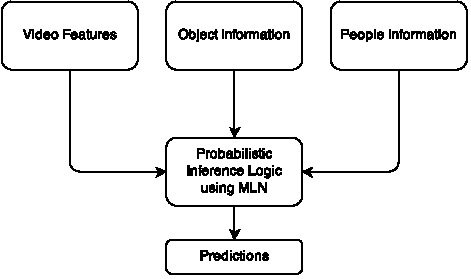
\includegraphics[scale=1.3]{approach} 
\caption{Approach of the Project}
\label{fig:approach}
\end{center}
\end{figure}

The video features are extracted as explained in section \ref{section_STIP}.
The code used in this phase is publicly made available at \cite{stipCode}.
Using one versus all (ovr) matlab interface of libsvm \cite{libsvm}, model is learnt to extract the 
confidence values from video feature classification.

The object features are evaluated using \cite{voc-release4}. 
Each object detection has a confidence value along with it.
This value is used to determine whether to consider detection
as a viable detection or spurious one. The thresholds for confidence
values are found experimentally. Details are given in chapter \ref{ch5_RESULTS}.

Main contribution of this project is in the formulation of
markov logic system. Alchemy \cite{alchemy2.0} software is
used to form markov logic network. The software allows convenient
representation of rules using first order logic and assigns weights to
such rules using the evidence provided. Following sections explain in detail
about the evidence creation, rules, etc.

\section{MLN Evidence}
The Hollywood2 data set \cite{hollywood2} (described in chapter \ref{ch5_RESULTS}) provides
true activity labels for training data. These labels are used to create predicates
like
\begin{equation}
	HasActivity( ``actioncliptrain00001", ``SitUp" )
\end{equation}

The learnt SVM model is used to classify training data set itself to get
confidence values of activities for all clips. These confidence values
are partitioned into bins to create predicates like
\begin{equation}
	\begin{split}
		~ & ActivityConf\_P1\_TO\_P15(``actioncliptrain00001",``SitUp") \\
		~ & ActivityConf\_NI\_TO\_N2(``actioncliptrain00002",``HandShake")
	\end{split}
\end{equation}

Here, P1\_TO\_P15 represents a bin with confidence value of +1 to +1.5.
Similarly other bins are formed and predicates are generated to form the evidence.
Each clip has 12 such predicates as there are 12 activity classes.

Object detector \cite{voc-release4} gives object detections in frames
along with the corresponding confidence values. Experimentally determined thresholds
are used to decide whether to consider object detection and predicates like following are formed
\begin{equation}
	\begin{split}
		~ & ObjPresent(``actioncliptrain00001",``person") \\
		~ & ObjPresent(``actioncliptrain00002",``car")
	\end{split}
\end{equation}

Finally, to generate evidence for people information, average number of ``person"
objects are calculated in each clip. These averages are partitioned into bins
and each clip is assigned one bin. Predicates like following are formed using this method
\begin{equation}
	\begin{split}
		~ & NumPersons\_1\_TO\_15(``actioncliptrain00001") \\
		~ & NumPersons\_0\_TO\_1(``actioncliptrain00002")
	\end{split}
\end{equation}





\section{MLN Rules}
For learning MLN model, rules corresponding to bins of confidence
from {\bf video classifier} are written.
For example,
\begin{equation}
	\begin{split}
		ActivityConf\_N1\_TO\_N05(clip,activity) \implies & HasActivity(clip,activity) \\
		ActivityConf\_P1\_TO\_P15(clip,activity) \implies & HasActivity(clip,activity)
	\end{split}
\end{equation}

Here, the $1^{st}$ rule captures relation between low confidence ($-1$ to $-0.5$) of presence
of activity and actual evidence. And $2^{nd}$ rule captures relation between
higher confidence ($+1$ to $+1.5$) of presence of activity and actual evidence.
Thus intuitively, $1^{st}$ rule will get lower weight as compared to $2^{nd}$ rule.

~ \\
For adding {\bf object information}, both positive and negative rules are written.
Positive rules are intuitive rules which enhance the probability of likely
inference. Negative rules are counter intuitive rules which suppress the
probability of unlikely rules. In both the types, the confidence of classification
improves. Below is example of few positive rules
\begin{equation}
	\begin{split}
		ObjPresent(c,``chair") \implies & HasActivity(c,``Eat") \\
		ObjPresent(c,``car") \implies & HasActivity(c,``DriveCar")
	\end{split}
\end{equation}
and few negative rules
\begin{equation}
	\begin{split}
		ObjPresent(c,``bus") \implies & HasActivity(c,``StandUp") \\
		ObjPresent(c,``car") \implies & HasActivity(c,``HandShake")
	\end{split}
\end{equation}

~ \\
For learning relationship between {\bf people information} and activities,
rules consisting of bins of number of people and activities are written.
For example,
\begin{equation}
	\begin{split}
		NumPersons\_0\_TO\_1(clip)\implies & HasActivity(clip,+a) \\
		NumPersons\_1\_TO\_15(clip)\implies & HasActivity(clip,+a)
	\end{split}
\end{equation}

where, $1^{st}$ rule has a bin that corresponds to average number of people 
per frame between 0 to 1.
``+a" means rule will be expanded to all possible activities. Thus for each bin,
rules corresponding to all 12 activities will be used in MLN learning.




\section{MLN Inference}
For inference, the learnt SVM model is used to classify testing
data set clips. This step provides with the confidence values of activities for
each clip. These confidence values are partitioned into bins in same manner
as done for generating evidence.
The object and people information is added in similar fashion as that of
evidence generation process. 

Inference is made on predicate ``HasActivity". Thus only difference
between evidence and inference is absence of ``HasActivity" predicates.

Sample inference instance looks like
\begin{equation}
	\begin{split}
		~ & ActivityConf\_P1\_TO\_P15(``actioncliptest00001",``Kiss") \\
		~ & ActivityConf\_N2\_TO\_N15(``actioncliptest00002",``Eat") \\
		~ & ObjPresent(``actioncliptest00001",``person") \\
		~ & ObjPresent(``actioncliptest00002",``person") \\
		~ & NumPersons\_2\_TO\_I(``actioncliptest00001") \\
		~ & NumPersons\_1\_TO\_15(``actioncliptest00002") \\
		~ & \vdots
	\end{split}
\end{equation}

~ \\
{\bf AAP Calculations - }Using the probabilities given by MLN inference, inferred activity for each
clip is determined corresponding to maximum probability. The data set provides with true activity labels for test clips. 
These true activities and MLN inferred activities are used to calculate average average precision
of MLN system. Next chapter shows the results.



\chapter{Results}

\label{ch5_RESULTS}
{\bf Data set - } All experiments in this project are performed on standard Hollywood2 (actions) 
\cite{hollywood2} data set from \cite{actionsInContext}. 
It has 823 labeled training video clips and 884 labeled testing video clips. 
There are 12 activity classes : AnswerPhone, DriveCar, Eat, FightPerson,
 GetOutCar, HandShake, HugPerson, Kiss, Run, SitDown, SitUp, StandUp.
 Each clip is 10 to 30 seconds long. Frame rate is 24 fps.
 Each clip is provided with a true label. Few of the clips have multiple labels, in this project, only single labelled clips are used.


 \section{Methodology}
 \label{section_METHODOLOGY}
 {\bf Video recognizer setup - } 100,000 HoG-HoF feature vectors are randomely sampled from 
 set of all feature vectors extracted from video clips using \cite{stipCode}.
 While doing random sampling, each clip is given equal chance - this avoids biased sampling
towards (or against) any particular class of videos if they happen to be longer (or shorter) than other videos on an average.
These randomely sampled descriptors are clustered in $k = 200$ clusters using k-means.
All clips are represented in Bag-of-Features representation over these clusters as explained in section \ref{section_BOF}.

~\\
{\bf SVM - } Matlab interface of libsvm \cite{libsvm} is used to train 
12 one-vs-rest (ovr) models corresponding to 12 activity classes. A RBF kernel is used with parameters, $\gamma = 0.01$ and $C = 100$.

~\\
{\bf Object Detector Setup - } Object detector explained in section \ref{section_OBJDET} is used. 
This run of object detection has a threshold of -0.9. 
Object specific thresholding is done at a later stage while forming evidence for MLN.

The visual output of object detector looks as shown in figures \ref{fig:CarDetection} and \ref{fig:PersonDetection}. 
The boxes are called as bounding boxes.
For each box, a confidence value is also evaluated.
Table \ref{table:ObjDetection} shows sample confidence output.

\floatstyle{plain}
\restylefloat{figure}
\begin{figure}[here]
\begin{center} 
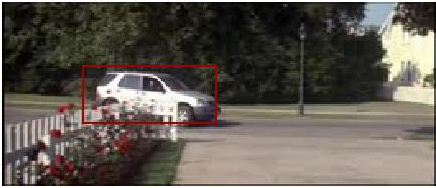
\includegraphics[scale=0.5]{car_detection_1.jpg} 
\caption{ Car detection in a frame. \label{fig:CarDetection}} 
\end{center} 
\end{figure}  

\begin{figure}[here]
\begin{center} 
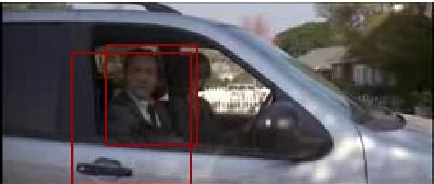
\includegraphics[scale=0.5]{person_detection_151.jpg} 
\caption{ Person detection in a frame. \label{fig:PersonDetection}} 
\end{center} 
\end{figure}  

\begin{table}[t,here]
\centering
\begin{tabular}{|l|c|}
\hline
\multicolumn{2}{|c|}{FRAME1} \\
\hline
 Car            &-0.181786\\
\hline
\multicolumn{1}{|c|}\vdots & \vdots \\
\hline
\multicolumn{1}{|c|}\vdots & \vdots \\
\hline
\multicolumn{2}{|c|}{FRAME151} \\
\hline
Person	&0.579786\\
\hline
Person	&-0.593087\\
\hline
\end{tabular}
\caption{Output of object detector with decision values}
\label{table:ObjDetection}
\end{table}

~ \\
{\bf Alchemy Setup - } MLN model is learnt using Alchemy 2.0 \cite{alchemy2.0} software.
All the parameters are kept default. `QueryEvidence' option is not set.

~\\
{\bf Classification metric - } Predictions are compared by taking \index{Average Average Precision|see {AAP}} average average precision as a measure.
As explained in \cite{actionsInContext}, average precision(AP) approximates area under recall-precision curve.
Thus, AP for each activity class is calculated and then finally averaged over all the classes, average AP (\index{AAP}AAP) is calculated.
AP is taken as a measure of performance in the work of \cite{actionsInContext}.

\section{Precision Comparisons}
{\bf MLN - } Using alchemy 2.0 \cite{alchemy2.0} software, various experiments were performed 
to add the object and people information to the existing video recognizer. 

\begin{table}[t,here]
\centering
\captionsetup{justification=centering,margin=2cm}
\begin{tabular}{| l | c | c | c | c | c |}
\hline
	{\bf Activity Class} & {\centering {\bf SVM}}
	&\multicolumn{4}{c|}{\centering {\bf MLN} }\\ \hline

	~ & ~
	& \multicolumn{1}{p{1.2cm}|}{\centering {\bf Only \\ Action}}
	& \multicolumn{1}{p{1.2cm}|}{\centering {\bf Action \& \\ Object}}
	& \multicolumn{1}{p{1.2cm}|}{\centering {\bf Action \& \\ People}}
	& \multicolumn{1}{p{1.2cm}|}{\centering {\bf Action \\ Object \& \\ People}}
	\\ \hline
	AnswerPhone	& 11.36\%  & 10.64\%  & 11.11\%  & 11.67\%  & 12.73\%  \\ \hline
	DriveCar  	& 66.96\%  & 66.06\%  & 66.67\%  & 71.57\%  & 68.18\%  \\ \hline
	Eat  		& 45.45\%  & 32.50\%  & 40.00\%  & 35.00\%  & 40.00\%  \\ \hline
	FightPerson  	& 57.63\%  & 56.90\%  & 54.84\%  & 61.54\%  & 62.26\%  \\ \hline
	GetOutCar  	& 17.86\%  & 8.00\%   & 13.79\%  & 17.39\%  & 14.29\%  \\ \hline
	HandShake  	& 25.93\%  & 21.43\%  & 25.00\%  & 30.77\%  & 41.67\%  \\ \hline
	HugPerson  	& 15.15\%  & 15.79\%  & 13.79\%  & 14.29\%  & 16.13\%  \\ \hline
	Kiss  		& 18.18\%  & 18.07\%  & 19.78\%  & 19.79\%  & 20.65\%  \\ \hline
	Run  		& 38.78\%  & 36.42\%  & 41.48\%  & 40.32\%  & 42.15\%  \\ \hline
	SitDown  	& 40.96\%  & 38.10\%  & 35.56\%  & 34.78\%  & 39.56\%  \\ \hline
	SitUp  		& 5.26\%   & 0.00\%   & 5.26\%   & 0.00\%   & 12.50\%  \\ \hline
	StandUp  	& 35.20\%  & 38.46\%  & 36.29\%  & 38.26\%  & 36.24\%  \\ \hline
	AAP  		& 31.56\%  & 28.53\%  & 30.30\%  & 31.28\%  & 33.86\%  \\ \hline

\end{tabular}
\caption{MLN Experiments - Average precisions}
\label{table:MLN_RESULTS}
\end{table}



TODO - Explanation of above table.



~\\

{\bf TF-IDF Features - }
The Bag-of-Features vector of each clip can be appended with Term Frequency -
Inverse Document Frequency (tf-idf) features corresponding 
to 12 objects and number of people information. Thus adding 13 more features to each
feature vector.
These new feature vectors are now used to learn SVM model with similar parameters 
and methodology explained in section \ref{section_METHODOLOGY}.
It shows significant improvemnt as described in table \ref{table:SVM_TFIDF}.

\begin{table}[t,here]
\centering
\captionsetup{justification=centering,margin=2cm}
\begin{tabular}{| l | c | c |}
\hline
	{\bf Activity Class}
	& \multicolumn{1}{p{3cm}|}{\centering {\bf AP - Basic \\ SVM}}
	& \multicolumn{1}{p{3cm}|}{\centering {\bf AP - Object \\ and People} }\\ \hline
AnswerPhone & 11.36\% & 16.67\% \\ \hline
DriveCar & 66.96\% & 70.09\% \\ \hline
Eat & 45.45\% & 50.00\% \\ \hline
FightPerson & 57.63\% & 66.04\% \\ \hline
GetOutCar & 17.86\% & 12.12\% \\ \hline
HandShake & 25.93\% & 31.82\% \\ \hline
HugPerson & 15.15\% & 17.86\% \\ \hline
Kiss & 18.18\% & 20.69\% \\ \hline
Run & 38.78\% & 39.35\% \\ \hline
SitDown & 40.96\% & 42.05\% \\ \hline
SitUp & 5.26\% & 8.70\% \\ \hline
StandUp & 35.20\% & 37.88\%\\ \hline
Average AP & 31.56\% & 34.44\% \\ \hline
%
\end{tabular}
\caption{Average precision after adding tf-idf features}
\label{table:SVM_TFIDF}
\end{table}

TODO - Comparison between tf-idf and MLN. Feedback.

\begin{comment}
Table \ref{table:SVM_Setup} shows APs for all classes as per SVM setup of this project.

\begin{table}[t,here]
\centering
\captionsetup{justification=centering,margin=2cm}
\begin{tabular}{| l | c | c |}
\hline
{\bf Activity Class} & {\bf AP as per Paper} & {\bf AP as per project} \\ \hline
%
AnswerPhone & 8.80\% & 11.36\% \\ \hline
DriveCar & 74.90\% & 66.96\% \\ \hline
Eat & 26.30\% & 45.45\% \\ \hline
FightPerson & 67.50\% & 57.63\% \\ \hline
GetOutCar & 9.00\% & 17.86\% \\ \hline
HandShake & 11.60\% & 25.93\% \\ \hline
HugPerson & 13.50\% & 15.15\% \\ \hline
Kiss & 49.60\% & 18.18\% \\ \hline
Run & 53.70\% & 38.78\% \\ \hline
SitDown & 31.60\% & 40.96\% \\ \hline
SitUp & 7.20\% & 5.26\% \\ \hline
StandUp & 35\% & 35.20\% \\ \hline
Average AP & 32.39\% & 31.56\% \\ \hline
%
\end{tabular}
\caption{Average precision for Basic SVM Setup - without using tf-idf features}
\label{table:SVM_Setup}
\end{table}
\end{comment}


\chapter{Conclusion}

\label{ch6_CONCLUSION}

Various experiments aimed at improving video activity recognition were performed during this project.
Approaches included experiments using MLNs and adding object \& people information to SVM learning.
We provide a seamless method to combine outputs of multiple noisy detectors to enhance the recognition
process. It was found that adding object and people information to the existing recognition framework
improves the precision results.

%Moreover, wherever there is a relationship between action and object, that can be represented by first order logic,
% markov logic networks effectively capture the relationship.

The system developed by this project builds on top of video recognizer and object detector.
Higher the precision of both of these systems, higher the precision of overall system.

Future work can target to add more semantic information to the model such as scene information.
An important future contribution could be to complete feed-back loop to improve the quality
of the object detector. 
For instance, if dining table is occluded in a video of `eating' activity, the feedback from 
the activity recognizer can be used to boost up the confidence and predict the presence of dining table.

\begin{comment}
For instance, if dining table is occluded in `eating' activity,
the feedback information from MLN can be used to increase the confidence of the presence of
object dining table.
\end{comment}


\bibliographystyle{plain}
\bibliography{biblio}

%\appendix
%\begin{appendices} % Using appendices environment for more functunality
%\chapter{CHAPTER NAME}

\section{SECTION NAME}
\lipsum[1]

\section{SECTION NAME}
\lipsum[2]
%\end{appendices}

\printindex
\end{document}
	
